\section{Modelo del mapa}

Representamos al entorno donde se desplaza el robot mediante una cuadrícula regular de celdas cuadradas. Cada celda se clasifica como libre, ocupada, obstáculo u borde. La cuadrícula se presenta en el programa como la matriz de la figura \ref{fig:map_definition}, facilitando su tratamiento mediante algoritmos de planificación y control. Durante el movimiento del robot, los sensores actualizan dinámicamente el estado de localización del robot y de ocupación de las celdas.

\begin{figure}[htpb]
   \centering
   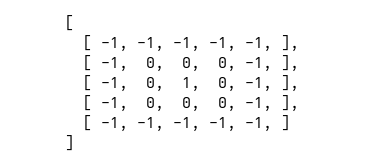
\includegraphics[width=0.8\linewidth]{images/map_definition_matriz.png}
   \caption{Matriz que define el mapa y sus elementos para el programa en Python}
   \label{fig:map_definition}
\end{figure}

Los colores de referencia utilizados en la interfaz del mapa son: rojo para bordes, blanco para obstáculos, gris para celdas libres y otro color para el robot, tal como se observa en la figura \ref{fig:modelomapa}. La odometría del robot convierte su posición en coordenadas métricas, alineadas con el centro de las celdas.

\begin{figure}[htpb]
    \centering
    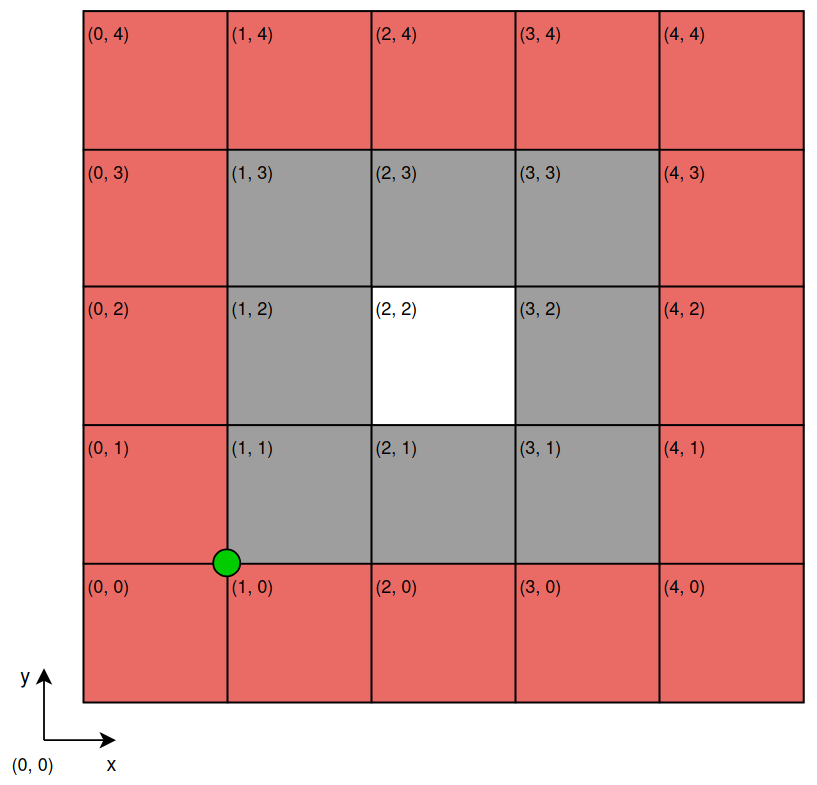
\includegraphics[width=1.0\linewidth]{images/modelo_del_mapa.png}
    \caption{Modelo del mapa en dos dimensiones donde cada celda esta identificada con un par de coordenadas}
    \label{fig:modelomapa}
\end{figure}

\subsection{Calculador de trayectorias}

Para la planificación de rutas empleamos el algoritmo $A*$ por su eficiencia y capacidad para encontrar el camino más corto entre dos puntos. Este algoritmo combina el costo acumulado desde el origen $g(n)$ con una heurística $h(n)$ que estima la distancia restante hacia el destino (ecuación \ref{ec:distancia}). En este caso, utilizamos la distancia de Manhattan como heurística, adecuada para movimientos ortogonales en una grilla, ya que es equivalente a calcular la distancia desplazándose en línea recta, primero en una dirección ($x$) y luego en otra ($y$) como si se caminara por las calles de Manhattan donde se tiene un patrón cuadriculado. \cite{sariffpathplan} \cite{cuevaspathfinding}

\begin{equation}
    f(n) = g(n) + h(n)    
    \label{ec:distancia}
\end{equation}

El algoritmo comienza con la celda inicial, que se agrega a una lista abierta (open list) de celdas por explorar. En cada paso, el algoritmo selecciona la celda con el valor $f(n)$ más bajo de la lista abierta y la mueve a una lista cerrada (closed list) de celdas ya exploradas. Luego, evalúa las celdas vecinas de la celda actual. Si una celda vecina no está en la lista cerrada y no hay una ruta mejor a esa celda en la lista abierta, se actualizan sus valores de $g$, $h$ y $f$ , y se agrega a la lista abierta. Este proceso se repite, seleccionando y evaluando celdas hasta que se alcanza la celda destino.

\subsection{Red de Petri}
Este trabajo tiene por objetivos el control, seguimiento del comportamiento y modelado de un sistema compuesto por una flota de robots donde cada uno tiene que seguir una trayectoria definida y calculada utilizando el algoritmo $A*$ determinando el camino más corto hacia su destino. Teniendo esto en mente, es necesaria la implementación de un método para evitar los problemas inherentes en los sistemas multi-robot: las colisiones entre los robots y los bloqueos del sistema, haciendo que algunos robots no puedan terminar su trayectoria y por lo tanto, entorpecer todo el sistema. Esta iniciativa surge al encarar el proyecto como un sistema multi-robot, lo cual no se había planteado antes en los modelos previos de la familia Hermes y presenta una novedad para las futuras implementaciones.

Al tener el conjunto de trayectorias definidas para cada robot, se modela el sistema y el mapa mediante el uso de Redes de Petri, que no son más que representaciones matemáticas con una simbología gráfica de un sistema de eventos discretos. El entorno en el cual se mueven los robots se considera particionado el mapa en regiones (celdas) y cada región del mapa se modela como una plaza en la Red de Petri. Para evitar las colisiones entre los robots, establecemos regiones con capacidad finita (recursos), donde no pueden pasar por ellas más robots de los recursos definidos. \cite{mahulea2020multi}

\subsection{Método de imposición sobre Global Interpreter Lock}
La concurrencia en Python está influenciada y controlada por el \textit{Global Interpreter Lock (GIL)}, que impide a múltiples hilos ejecutar código Python puro en paralelo dentro de un mismo proceso.

Este proyecto está pensado para que escale en cantidad de robots, y controlemos una flota de ellos, por lo tanto, cada hilo en Python va a representar un robot, cuya gestión va a estar coordinada a través del monitor basado en una Red de Petri.

Garantizamos un control ordenado de los hilos mediante la implementación de un mecanismo de sincronización mediante Lock, permitiendo bloquear el hilo de un robot cuando éste no puede avanzar y continuar con los demás. Este enfoque asegura una ejecución eficiente dentro del marco definido por la red de Petri, optimizando el flujo de trabajo sin afectar la estabilidad del sistema.

Por todo lo anterior implementamos un método donde le asignamos una prioridad a un determinado hilo en base a la política y, por lo tanto, el Monitor puede elegir cuál va a ser el siguiente hilo a ejecutar. Interpretamos esto como la imposición sobre el mecanismo $GIL$, mejorando el manejo fino de hilos forzando el siguiente hilo a ejecutar.

\subsection{Modelo del mapa en Red de Petri}

El controlar de forma efectiva los lugares que ocupa el robot en el mapa es esencial para que pueda completar su recorrido, es por ello que modelamos el mapa como una Red de Petri, donde cada celda transitable se representa como una plaza, y cada nueva posición que ocupa en el mapa es un marcado diferente en la red. Incorporamos plazas adicionales que representan los recursos compartidos: cada región con capacidad unitaria incluye un lugar de recurso con una única marca, que permite o bloquea el ingreso de un nuevo robot. Esto se observa con claridad en la figura \ref{fig:rdp_no_grid}, ya que es el modelo de mapa de la figura \ref{fig:map_definition} pero representado como una red de Petri.

\begin{figure}[htpb]
   \centering
   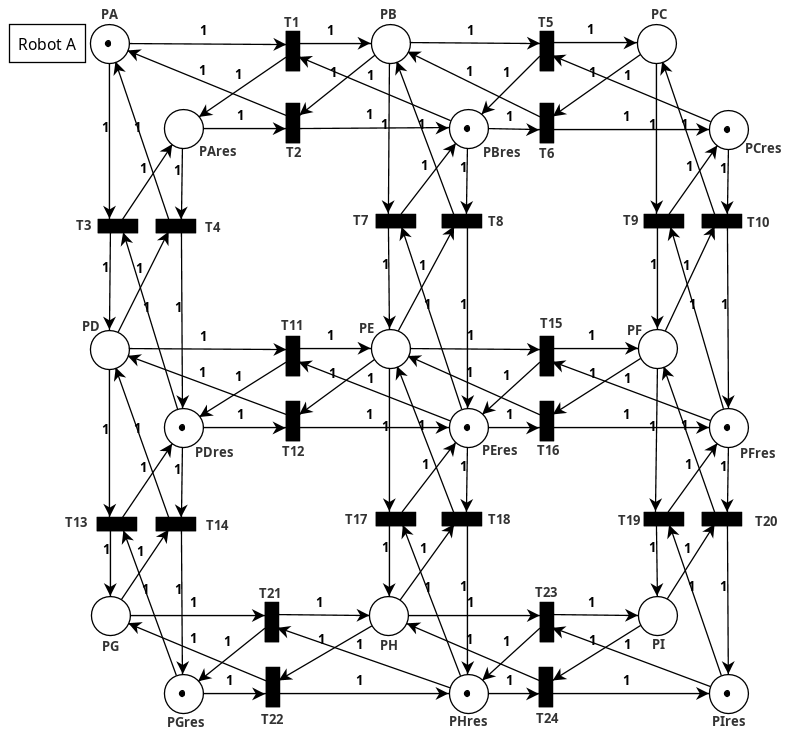
\includegraphics[width=0.9\linewidth]{images/rdp_no_grid.png}
   \caption{Representación del mapa en una red de Petri generado en el software Petrinator \cite{petrinator}}
   \label{fig:rdp_no_grid}
\end{figure}

Este modelo permite garantizar la propiedad de exclusión mutua en regiones críticas y facilita el análisis estructural del sistema. La red se genera a partir de un archivo de texto que describe el mapa, y se traduce en una matriz de incidencia y un vector de marcado inicial. Esto lo hace un sistema escalable, seguro y adaptable a distintos entornos. \cite{mahulea2020multi}

\subsection{Monitor}

La manera en que controlamos la ocupación de los espacios en el mapa, es decir, cómo evoluciona la trayectoria de cada robot, es mediante el disparo de un Monitor. Este es el que va a controlar, guiar y realizar la toma de decisiones para que cada robot pueda seguir su trayectoria sin interrumpir a los demás y por lo tanto no bloquear todo el sistema. Para guiar a cada robot en su trayectoria, cada uno va a estar representado por un hilo lógico dentro del programa. 

Entonces, cuando un robot desea avanzar, consulta al Monitor, que verifica si la transición está habilitada y, en caso de múltiples solicitudes, aplica una política de prioridad. \cite{papermico}.

Llevamos a cabo la validación del Monitor utilizando la Red de Petri Productor-Consumidor con 1 millón de disparos, verificando en cada uno la consistencia de P-invariantes y T-invariantes.

\subsubsection{Detección y resolución de conflictos}

Los conflictos son detectados cuando múltiples robots intentan acceder a la misma celda en el mismo momento cómo se muestra en la figura \ref{fig:conflicto_map}. En tal caso, activamos una política de prioridad que favorece al robot con menor cantidad de celdas restantes por recorrer. 

\begin{figure}[htpb]
    \centering
    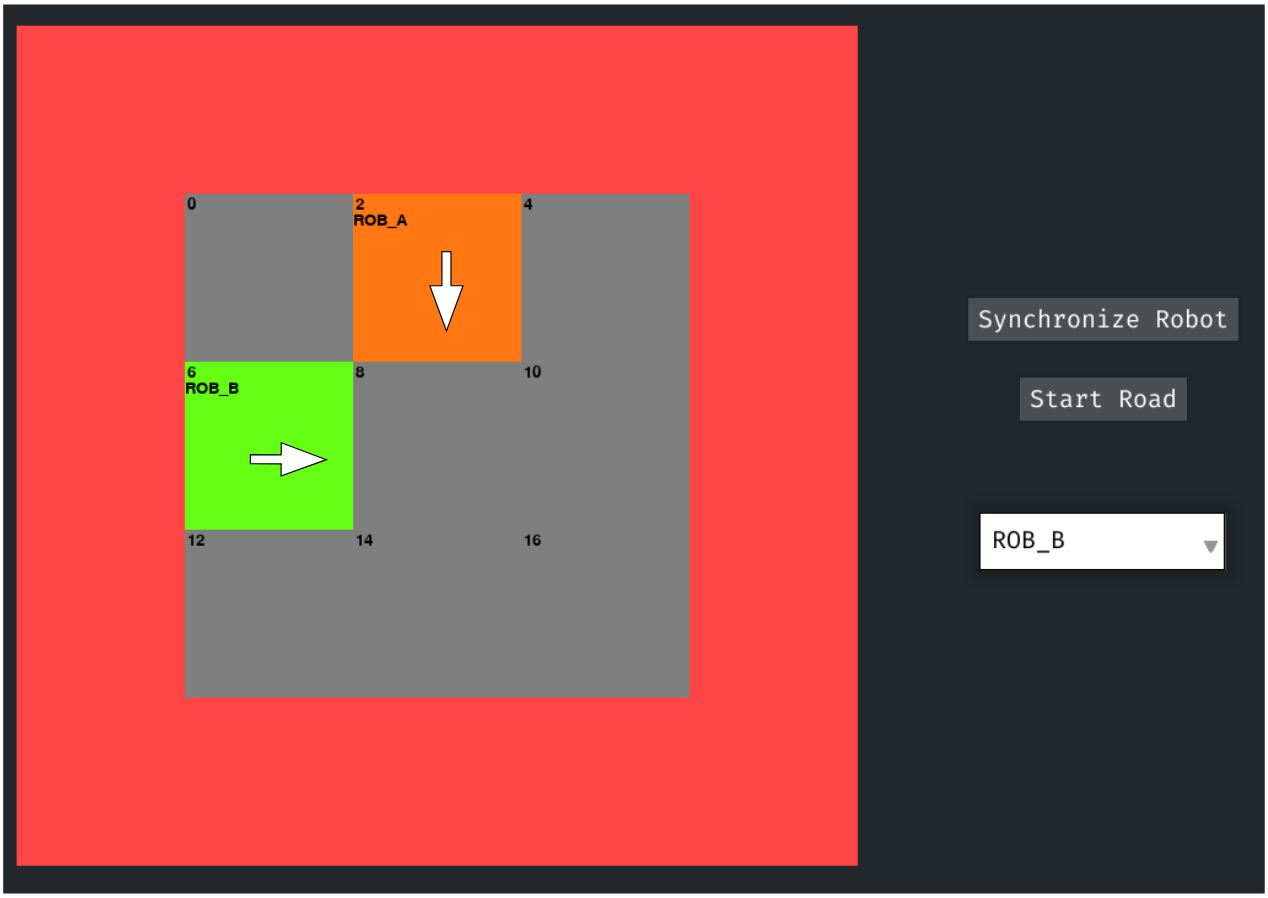
\includegraphics[width=1.0\linewidth]{images/conflicto_map.png}
    \caption{Representación de un conflicto entre dos robots que intentan pasar por la misma celda}
    \label{fig:conflicto_map}
\end{figure}

Si existe una situación en donde dos robots intentan intercambiar lugares, activamos una política de re-planificación que penaliza al robot con mayor camino restante. Este conflicto se contempla en la figura \ref{fig:conflicto_path}.

\begin{figure}[htpb]
    \centering
    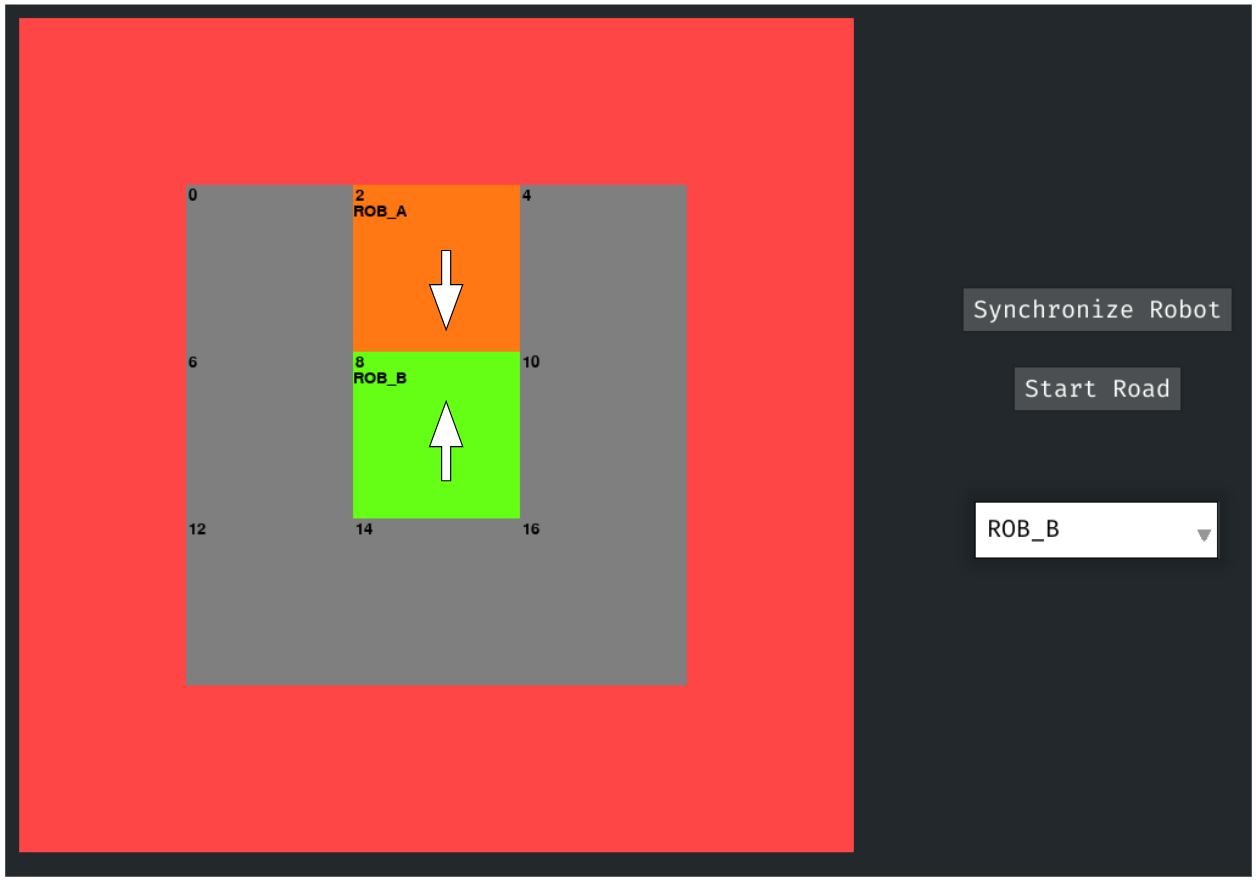
\includegraphics[width=1.0\linewidth]{images/conflicto_path.png}
    \caption{Situación de conflicto en donde dos robots intentan intercambiar lugares}
    \label{fig:conflicto_path}
\end{figure}

Para garantizar un flujo ordenado, el monitor mantiene una cola de cortesía tipo FIFO que regula el acceso de los hilos a los recursos. La implementación fue validada mediante simulaciones sobre redes estándar (Productor-Consumidor) y pruebas integradas con el sistema físico, demostrando la efectividad del modelo y la robustez del monitor ante conflictos concurrentes.